\def\pgfsysdriver{pgfsys-dvisvgm.def}
\documentclass[tikz,border=2pt]{standalone}
\usepackage{amsmath}
\usepackage{tikz}
\usetikzlibrary{arrows.meta, positioning, calc, fit}

\definecolor{perilText}{HTML}{1A1A1A}
\definecolor{perilMuted}{HTML}{71717A}
\definecolor{perilAccent}{HTML}{9B8AB8}
\definecolor{perilSurface}{HTML}{EAE8E3}
\definecolor{perilBg}{HTML}{F5F3EF}

\begin{document}
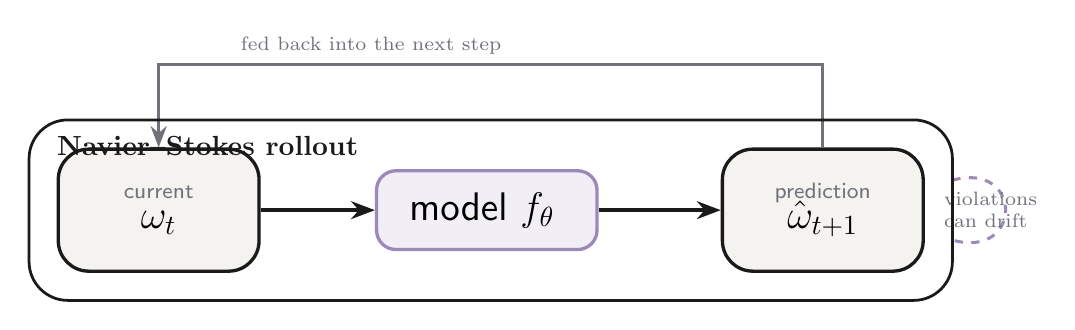
\begin{tikzpicture}[
    font=\sffamily,
    >=Stealth,
    state/.style={
        draw=perilText,
        line width=1.2pt,
        rounded corners=11pt,
        fill=perilBg,
        minimum width=2.55cm,
        minimum height=1.55cm,
        align=center
    },
    model/.style={
        draw=perilAccent,
        line width=1.2pt,
        rounded corners=7pt,
        fill=perilAccent!14,
        minimum width=2.80cm,
        minimum height=1.00cm,
        align=center
    },
    arrow/.style={->, line width=1.25pt, draw=perilText},
    feedback/.style={->, line width=1.05pt, draw=perilMuted},
    drift/.style={line width=1.1pt, draw=perilAccent, dashed},
]

\node[state] (current) at (0,0) {
    {\footnotesize\color{perilMuted}current}\\[-1pt]
    {\Large $\omega_t$}
};

\node[model, right=1.45cm of current] (model) {
    {\Large model $f_\theta$}
};

\node[state, right=1.55cm of model] (pred) {
    {\footnotesize\color{perilMuted}prediction}\\[-1pt]
    {\Large $\hat{\omega}_{t+1}$}
};

\draw[arrow] (current) -- (model);
\draw[arrow] (model) -- (pred);

\draw[feedback]
    (pred.north) -- ++(0,1.05)
    -| node[pos=0.34, above, font=\scriptsize, color=perilMuted]
        {fed back into the next step}
    (current.north);

\draw[drift] ($(pred.east)+(0.35,0.38)$)
    .. controls +(0.90,0.25) and +(0.90,-0.25) ..
    ($(pred.east)+(0.35,-0.38)$);
\node[align=left, font=\scriptsize, color=perilMuted, right=0.12cm of pred.east]
    {violations\\can drift};

\node[
    draw=perilText,
    rounded corners=14pt,
    line width=1pt,
    inner sep=0.35cm,
    fit=(current)(model)(pred)
] (box) {};

\node[anchor=west, font=\bfseries, color=perilText]
    at ($(box.north west)+(0.25,-0.35)$) {Navier--Stokes rollout};

\end{tikzpicture}
\end{document}
